\documentclass[12pt]{report}

% Čeština
\usepackage[utf8]{inputenc}
\usepackage[IL2]{fontenc}
\usepackage[czech]{babel}

% Formát dokumentu
\usepackage{caption}
\usepackage{indentfirst}
\usepackage{graphicx}
\usepackage{textcomp}
\usepackage{amsmath}
\usepackage{parskip}
\usepackage{xspace}
\graphicspath{{img/}}
\usepackage[
left=30mm, 
right=30mm, 
top=30mm, 
bottom=30mm,
]{geometry}

% odstavec
\newcommand\myindent[1]{						
	\setlength\parindent{5mm}
	#1
	\setlength\parindent{0mm}
}											

\begin{document}
	
	% Titulní strana
	\begin{titlepage}
		\centering
		\Large
		
		
\includegraphics[width=.7\textwidth]{fav}
		
		\vspace{15mm}
		{\Huge\bfseries Hangman klient a server}
		
		\vspace{15mm}
		{\LARGE Semestrální práce KIV/UPS}
		
		\vfill
		\raggedright
		Mikuláš Mach\\
		mimach@students.zcu.cz\\
		A21B0202P
		\hfill 
		\today
	\end{titlepage}
	
	% Obsah
	\tableofcontents
	
	\chapter{Princip hry}
	\section{Obecná pravidla hry}
		Hangman neboli šibenice je hra, ve které je úkolem uhodnout předem určené slovo. Hádá se po jednotlivých písmenech a při každém špatném pokusu o uhodnutí písmena je hráči odebrán život. Hráč vyhrává, když uhodne celé slovo před tím než přijde o všechny životy
	\section{Implementace pravidel hry}
		Hra je implementována tak, aby šla hrát ve 2 až 4 hráčích. Hráč vyhrává, když jako první uhádne poslední dosud neuhodnuté písmeno z hádaného slova nebo když zůstane jako poslední naživu.

	%-------------------------
	%	Komunikační protokol
	%-------------------------
	
	\chapter{Komunikační protokol}
	
	\section{Popis komunikačního protokolu}
		Dle požadavků je protokol transparentní, tudíž nešifrovaný. Klient posílá vždy zprávu s daným formátem. Zpráva vždy začíná klíčovým slovem. Na každou zprávu od klienta existuje odpověď od serveru. Na obrázku \ref{fig:diagram} je ukázána komunikace klienta se serverem a jak se mění stav klientského objektu na serveru.
		
	\begin{figure}[h]
		\centering
		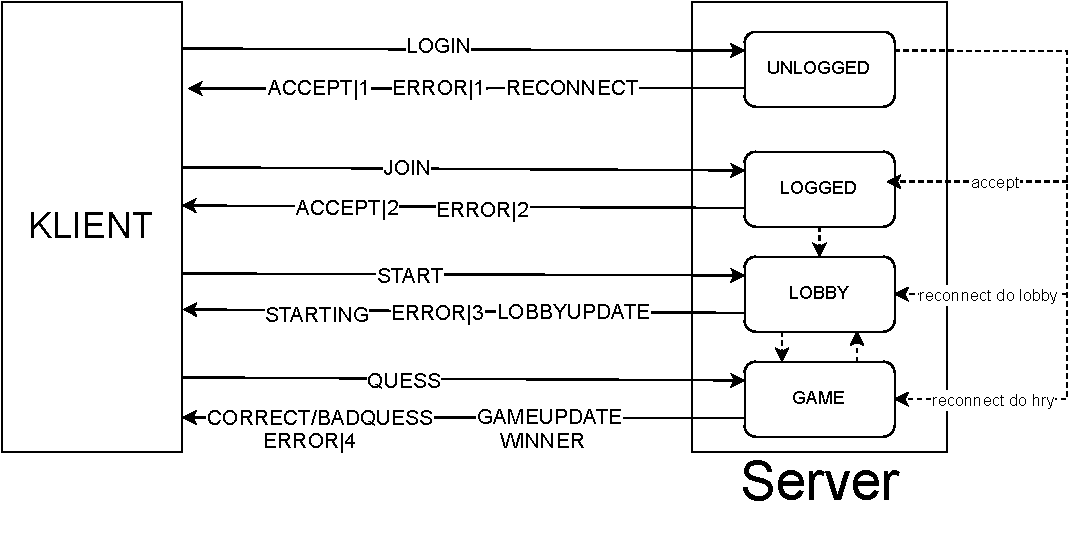
\includegraphics[width=.9\textwidth]{img/ups_diagram}
		\caption{Diagram komunikace}
		\label{fig:diagram}
	\end{figure}

	\section{Klientovy zprávy}
		\subsection{LOGIN}
		
		\begin{itemize}
			\item Formát: \textbf{LOGIN{\textbar}{\textless}jméno{\textgreater}}
			\item Server tuto zprávu přijme pouze když objekt klienta na serveru je ve stavu UNLOGGED
			\item \textbf{Odpověď} při správném připojení: \textbf{ACCEPT{\textbar}1{\textbar}{\textless}ping interval{\textgreater}{\textbar}{\textless}ping hranice{\textgreater}}
			
			\begin{itemize}
				\item {\textless}ping interval{\textgreater} - v jakém intervalu bude server zasílat zprávu PING
				\item {\textless}ping hranice{\textgreater} - po kolika neodpovězených zprávách PING bude klient úplně odpojen
			\end{itemize} 
			\item \textbf{Odpověď} při reconnectu: \textbf{RECONNECT{\textbar}{\textless}stav{\textgreater}{\textbar}{\textless}ping interval{\textgreater}{\textbar}{\textless}ping hranice{\textgreater}}
			\begin{itemize}
				\item {\textless}stav{\textgreater} - do jakého stavu se klient připojí, buď LOBBY nebo GAME
			\end{itemize} 
			\item \textbf{Odpověď} při odmítnutí: \textbf{ERROR{\textbar}1}
			\item \textbf{Odpověď} při duplicitě jména: \textbf{ERROR{\textbar}1{\textbar}1}
		\end{itemize}
	
	\subsection{JOIN}
		\begin{itemize}
			\item Formát: \textbf{JOIN}
			\item Touto zprávou klient žádá server, aby byl připojen do prvního volného lobby
			\item Server tuto zprávu přijme pouze když objekt klienta na serveru je ve stavu LOGGED
			\item \textbf{Odpověď}:  \textbf{ACCEPT{\textbar}2}
			\item \textbf{Odpověď} při odmítnutí: \textbf{ERROR{\textbar}2}
		\end{itemize}
	
	\subsection{START} 		
		\begin{itemize}
			\item Formát: \textbf{START}
			\item Touto zprávou klient žádá server o nastartování hry
			\item Server tuto zprávu přijme pouze když objekt klienta na serveru je ve stavu LOBBY a v daném lobby jsou aspoň 2 klienti
			\item \textbf{Odpověď}:  \textbf{STARTING{\textbar}{\textless}počáteční životy{\textgreater}{\textbar}{\textless}délka slova{\textgreater}{\textbar}{\textless}hráč na tahu{\textgreater}}
			
			\begin{itemize}
				\item {\textless}počáteční životy{\textgreater} - životy klientů na počátku hry
				\item {\textless}délka slova{\textgreater} - délka slova, které je v dané hře hádáno
				\item {\textless}hráč na tahu{\textgreater} - jméno hráče, který je jako první na tahu
			\end{itemize}
			
			\item \textbf{Odpověď} při odmítnutí: \textbf{ERROR{\textbar}3}
		\end{itemize}
	
	\subsection{QUESS}
		\begin{itemize}
			\item Formát: \textbf{QUESS{\textbar}{\textless}písmeno{\textgreater}}
			\item Klient se pokouší uhodnout jedno písmeno z hádaného slova
			\item Server tuto zprávu přijme pouze když objekt klienta na serveru je ve stavu ON\_TURN
			\begin{itemize}
				\item {\textless}písmeno{\textgreater} - jedno velké písmeno A-Z (bez háčků a čárek)
			\end{itemize}
			\item \textbf{Odpověď} při správném uhodnutí: \textbf{CORRECTQUESS{\textbar}{\textless}písmeno{\textgreater};{\textless}index{\textgreater}}
			\begin{itemize}
				\item {\textless}index{\textgreater} - index uhodnutého písmena ve slově
				\item jedno písmeno může mít více indexů, v tom případě budou indexy za sebou odděleny znakem \textbf{;}
				\item \textbf{tato odpověď je zaslána všem v dané hře}
			\end{itemize}
			\item \textbf{Odpověď} při neuhodnutí: \textbf{BADQUESS{\textbar}{\textless}jméno{\textgreater};{\textless}životy{\textgreater}{\textbar}{\textless}nový hráč na tahu{\textgreater}}
			\begin{itemize}
				\item {\textless}jméno{\textgreater} - jméno hráče, který neúspěšně hádal
				\item {\textless}životy{\textgreater} - aktuální stav životů po neuhodnutí
				\item {\textless}nový hráč na tahu{\textgreater} - jméno hráče, který je jako další na tahu
				\item \textbf{tato odpověď je zaslána všem v dané hře}
			\end{itemize}
			\item \textbf{Odpověď} při odmítnutí: \textbf{ERROR{\textbar}4}
		\end{itemize}
	
	\section{Zprávy od serveru}
	
		\subsection{PING}
			\begin{itemize}
				\item Formát: \textbf{PING}
				\item Odpověď od klienta: \textbf{PONG}
			\end{itemize}
		\subsection{LOBBYUPDATE}
			\begin{itemize}
				\item Formát: \textbf{LOBBYUPDATE{\textbar}{\textless}jméno{\textgreater};{\textless}stav připojení{\textgreater}{\textbar}.....}
					\begin{itemize}
						\item {\textless}stav připojení{\textgreater} 0 - hráč je připojen, 1 - hráč je dočasně nedostupný
						\item každá zpráva LOBBYUPDATE má 1 až 4 dvojice {\textless}jméno{\textgreater};{\textless}stav připojení{\textgreater}, každá dvojice je oddělena pomocí {\textbar}
						\item tato zpráva je zaslána všem klientům, kteří se nacházejí v lobby, ve kterém došlo k nějaké změně (např. odpojení nebo připojení hráče)
					\end{itemize}
			\end{itemize}
		\subsection{GAMEUPDATE}
			\begin{itemize}
				\item Formát: \textbf{GAMEUPDATE{\textbar}{\textless}jméno{\textgreater};{\textless}počet životů{\textgreater};{\textless}stav připojení{\textgreater}{\textbar}...!{\textless}hřáč na tahu{\textgreater}}
				\begin{itemize}
					\item {\textless}hřáč na tahu{\textgreater} - jméno hráče, který je aktuálně na tahu
					\item Stejný princip jako u zprávy LOBBYUPDATE, akorát tato zpráva navíc zasílá aktuální životy daného uživatele
				\end{itemize}
			\end{itemize}
		\subsection{QUESSED}
			\begin{itemize}
				\item Formát: \textbf{QUESSED{\textbar}{\textless}délka slova{\textgreater}{\textbar}{\textless}písmeno{\textgreater};{\textless}index{\textgreater};...{\textbar}...}
				\begin{itemize}
					\item Tato zpráva je zaslána klientovi, který se po výpadku opět připojil do hry, aby dostal aktuální stav uhodnutých písmen v hádaném slově
					\item Každé písmeno může mít více indexů a ve zprávě může být víc písmen
					\item příklad: QUESSED{\textbar}{\textless}délka slova{\textgreater}{\textbar}{\textless}písmeno{\textgreater};{\textless}index{\textgreater};{\textless}index{\textgreater}{\textbar}{\textless}písmeno{\textgreater};{\textless}index{\textgreater}
					\item písmena pouze A-Z (bez háčků a čárek)
				\end{itemize}
			\end{itemize}
		\subsection{WINNER}
			\begin{itemize}
				\item Formát: \textbf{WINNER{\textbar}{\textless}jméno{\textgreater}{\textbar}{\textless}slovo{\textgreater}}
				\begin{itemize}
					\item Zpráva je zaslána všem v dané hře
					\item zpráva obsahuje jméno vítěze a slovo, které bylo hádáno
				\end{itemize}
			\end{itemize}
		
		\newpage
		
		\section{Shrnutí zpráv}
		\begin{table}[htbp]
			\centering
			\begin{tabular}{c|c}
				\hline
				Klient posílá & Server odpovídá (jedna zpráva z bloku)\\
				\hline
				LOGIN{\textbar}{\textless}jméno{\textgreater} & ACCEPT{\textbar}1{\textbar}{\textless}ping interval{\textgreater}{\textbar}{\textless}ping hranice{\textgreater} \\
				&RECONNECT{\textbar}LOBBY{\textbar}{\textless}ping interval{\textgreater}{\textbar}{\textless}ping hranice{\textgreater} \\
				&RECONNECT{\textbar}GAME{\textbar}{\textless}ping interval{\textgreater}{\textbar}{\textless}ping hranice{\textgreater} \\
				& ERROR{\textbar}1\\
				& ERROR{\textbar}1{\textbar}1\\
				\hline
				JOIN & ACCEPT{\textbar}2 \\
				& ERROR{\textbar}2 \\
				\hline
				START & STARTING{\textbar}{\textless}počáteční životy{\textgreater}{\textbar}{\textless}délka slova{\textgreater}{\textbar}{\textless}hráč na tahu{\textgreater} \\
				& ERROR{\textbar}3\\
				\hline
				QUESS{\textbar}{\textless}písmeno{\textgreater} & CORRECTQUESS{\textbar}{\textless}písmeno{\textgreater};{\textless}index{\textgreater}... \\
				& BADQUESS{\textbar}{\textless}jméno{\textgreater};{\textless}životy{\textgreater}{\textbar}{\textless}nový hráč na tahu{\textgreater} \\
				& ERROR{\textbar}4\\
				
			\end{tabular}
			\caption{Zprávy co posílá klient.}
			\label{tab:klient-msg}
		\end{table}
		
		\begin{table}[htbp]
			\centering
			\begin{tabular}{c|c}
				\hline
				Server posílá & Klient odpovídá\\
				\hline
				PING & PONG \\
				
				\hline
				LOBBYUPDATE{\textbar}{\textless}jméno{\textgreater};{\textless}stav připojení{\textgreater}... &  \\
				\hline
				GAMEUPDATE{\textbar}{\textless}jméno{\textgreater};{\textless}počet životů{\textgreater};{\textless}stav připojení{\textgreater}...!{\textless}hřáč na tahu{\textgreater} &  \\
				\hline
				QUESSED{\textbar}{\textless}délka slova{\textgreater}{\textbar}{\textless}písmeno{\textgreater};{\textless}index{\textgreater}... ... &  \\
				\hline
				WINNER{\textbar}{\textless}jméno{\textgreater}{\textbar}{\textless}slovo{\textgreater}
				
				
			\end{tabular}
			\caption{Zprávy co posílá server.}
			\label{tab:server-msg}
		\end{table}
	
	\begin{table}[htbp]
		\centering
		\begin{tabular}{c|c}
			\hline
			Formát & Význam\\
			\hline
			ERROR{\textbar}1{\textbar}1 & zpráva LOGIN zaslána ve špatném klientském stavu \\
			\hline
			ERROR{\textbar}1{\textbar}2 & špatný formát zprávy JOIN \\
			\hline
			ERROR{\textbar}1{\textbar}3 & neplatné uživatelské jméno \\
			\hline
			ERROR{\textbar}1{\textbar}4 & uživatelské jméno je již zabráno \\
			\hline
			ERROR{\textbar}2{\textbar}1 & zpráva JOIN zaslána ve špatném klientském stavu \\
			\hline
			ERROR{\textbar}2{\textbar}2 & špatný formát zprávy JOIN \\
			\hline
			ERROR{\textbar}3{\textbar}1 & zpráva START zaslána ve špatném klientském stavu\\
			\hline
			ERROR{\textbar}3{\textbar}2 & špatný formát zprávy START \\
			\hline
			ERROR{\textbar}3{\textbar}3 & v lobby je málo klientů pro nastartování hry\\
			\hline
			ERROR{\textbar}4{\textbar}1 & zpráva QUESS zaslána ve špatném klientském stavu\\
			\hline
			ERROR{\textbar}4{\textbar}2 & špatný formát zprávy QUESS
			
			
		\end{tabular}
		\caption{Číselník errorů.}
		\label{tab:server-msg}
	\end{table}
	%-------------------------
	%	Implementace
	%-------------------------
	
	\chapter{Implementace serveru}
	
	\section{Úvod}
	Pro tvorbu aplikace serveru byl použit programovací jazyk C++, zejména kvůli podpoře již implementovaných datových struktur, jako třeba string, hash mapa, vector, queue, list, atd...
	
	Obsluha více klientů byla implementována pomocí pseudoparalelizace použitím funkce \textbf{select()}. Díky tomuto postupu se program nemusí starat o kritické sekce, protože běží sekvenčně. Kostra komunikace byla použita z ukázky na cvičení.
	
	Server je členěn do tříd.
	
	\section{Třída server}
	
	Tato třída zajišťuje spuštění serveru. Dále přijímá příchozí zprávy od klientů pomocí funkce \textbf{select()} a kontroluje zda jsou všichni klienti dostupní. Obsahuje metodu pro dočasné a úplné odpojení hráče.
	
	\section{Třída ClientManager}
	
	Tato třída má v sobě uložené všechny klienty aktuálně připojené k serveru. Obsahuje metody pro přihlášení uživatele, smazání uživatele a pro znovupřipojení uživatele.
	
	\section{Třída GameManager}
	
	Tato třída má v sobě uloženy všechny započaté i nezapočaté hry. Stará se o připojování hráčů do her, kontrolu jejich pokusů o hádání, aktualizaci stavu hry a o vyhodnocení vítěze.
	
	\section{Třída MessageHandlerer}
	
	Tato třída přebírá příchozí komunikaci od třídy server a vyhodnocuje zda je validní. Pokud ano, reaguje na ní volání metod z ostatních tříd.
	
	\section{Třída Game}
	
	Tato třída uchovává jací klienti jsou v dané hře a stav hry.
	
	\section{Třida Client}
	
	Uchovává všechny potřebné data o klientovy. Například jeho jméno, socket, jeho stav nebo hru ve které právě je.
	
	\section{Třída Responder}
	
	Pomocí metody pošle zprávu danému klientovi.
	
	\section{main.cpp}
	
	Obsahuje spuštění aplikace a ověření parametrů příkazové řádky

	\chapter{Implementace klienta}
	
	
	\section{Úvod}
	
	Pro implementaci klienta byl zvolen programovací jazyk Python, zejména kvůli jeho jednoduchosti a kvůli tomu že je multiplatformní.
	
	Pro implementaci grafického rozhraní byla zvolena knihovna Tkinter, která je součásti pythonu.
	
	Klientská aplikace běží ve dvouch vláknech. Jedno obsluhuje uživatelské rozhraní a druhé obsluhuje všechnu komunikaci se serverem. V komunikačním vláknu je použitá funkce \textbf{select()}.
	
	\section{Třída MyApp}
	
	Obsahuje metody pro vytvoření jednotlivých scén, jejich zobrazení, přepínání a aktualizaci. Dále obsluhuje tlačítka a odesílá instrukce komunikačnímu vláknu.
	
	\section{Třída CommunicationHandlerer}
	
	Komunikuje se serverem, ověřuje validitu zpráv a kontroluje zda je server dostupný, pokud ne, pokouší se o znovupřipojení. Volá metody ze třídy MyApp pro aktualizaci stavu uživatelského rozhraní.
	
	\section{Třída Game}
	
	Uchovává informace o hře, ve které se klient nachází. 
	%-------------------------
	%	Uživatelská příručka
	%-------------------------			
	
	\chapter{Uživatelská příručka }
	
	\section{Přeložení serveru}
	
	Pro překlad je využit software \textbf{cmake}, \textbf{makefile} a \textbf{g++}. V kořenovém adresáři serveru použijeme příkaz \textbf{cmake}, který z CMakeLists.txt vytvoří \textbf{makefile}. Následně pomocí příkazu \textbf{make} vytvoříme spustitelná soubor hangman\_server.
	
	\section{Spuštění serveru}
	
	Popisované spouštění je pro platformu linux. V adresáři kde máme přeložený spustitelný soubor použijeme v terminálu příkaz: \textbf{./hangman\_server {\textless}ip\_adresa{\textgreater} {\textless}port{\textgreater}}
	
	\begin{itemize}
		\item {\textless}ip\_adresa{\textgreater} - ip adresa serveru
		\item {\textless}port{\textgreater} - port serveru
	\end{itemize}
	
	\section{Spuštění klienta}
	
	V adresáři kde se nachází soubor \textbf{main.py} spustíme pomocí konzole/terminálu příkaz: \textbf{python3 main.py}, aby tento postup fungoval, musí být na daném počítači nainstalován python3
	
	
	
	%-------------------------
	%	Závěr
	%-------------------------
	
	\chapter{Závěr}
	
	Cílem práce bylo vytvořit síťovou hru pro více hráčů, která bude dostatečně stabilní a bude správně reagovat na výpadky. Toto zadání se podařilo naplnit v plném rozsahu a výsledkem je realizace hry šibenice. Aplikace nepadají, nezasekávají se a reagují na požadavky hráčů. Server je určen pro operační systém Linux a aplikace klienta byla vytvořena pro operační systémy Windows 10 a Linux.
	
\end{document}